\autobookmark
\begin{frame}{Using Monte Carlo to simulate ASE}
  \begin{columns}
    \begin{column}{.5\textwidth}
      \begin{center}
       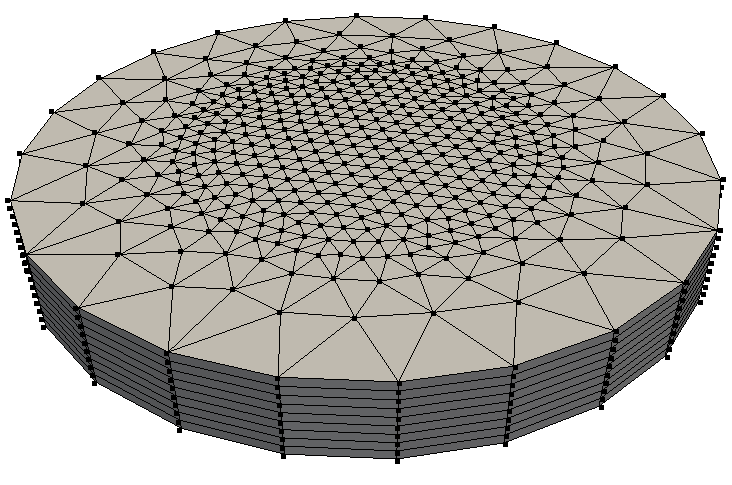
\includegraphics[height=0.25\paperheight]{graphics/samples_round.png}
      \end{center}
    \end{column}
    \begin{column}{.5\textwidth}
        The medium is sampled non-uniformly
    \end{column}
  \end{columns}

  \begin{itemize}
      \myuncover{2}{4}{
      \item
        ASE for one of the sample points can be determined:
        \begin{equation}
          \Phi_{ASE}(s_i)=\frac{1}{4\pi}\iint\limits_{V \lambda}
          \frac
          {\hat{n}(r)}
          {\tau_{f}|\rho(r,s_i)|^2}~g(\lambda)~G_{r\rightarrow
          s_i}~dV d\lambda
        \end{equation}
      }
      \myuncover{3}{4}{
      \item With MC, the problem can be transformed into a sum:
        \begin{equation}
          \Phi_{ASE}(s_i) = 
          \frac{1}{4\pi N\tau_f}
          \sum^{N}{1}_{u=0} \hat{n}(r_{i,u}) \cdot
          gain(\overrightarrow{r_{i,u}s_i})
        \end{equation}
      }
      \myuncover{4}{4}{
        \item This Monte Carlo integration can be solved by ray tracing
      }
  \end{itemize}
\end{frame}

%\begin{frame}{Predefined colours}
%  The template defines a set of colours according to the CD guidelines:\par
%  \begin{itemize}
%      \begin{minipage}[t]{0.5\linewidth}
%      \item \textcolor{hzdr-blue}{Helmholtz Blue}    
%      \item \textcolor{hzdr-orange}{Rossendorf Orange}  
%      \item \textcolor{hzdr-darkblue}{Helmholtz Dark Blue}
%      \item \textcolor{hzdr-gray1}{Gray1}   
%      \item \textcolor{hzdr-gray2}{Gray2}   
%      \item \textcolor{hzdr-gray3}{Gray3}   
%      \item \textcolor{hzdr-struct}{Structure of Matter}  
%      \end{minipage}%
%      \begin{minipage}[t]{0.5\linewidth}
%      \item \textcolor{hzdr-health}{Health}  
%      \item \textcolor{hzdr-energy}{Energy}  
%      \item \textcolor{hzdr-earth}{Earth and Environment}   
%      \item \textcolor{hzdr-keytec}{Key Technologies}  
%      \item \textcolor{hzdr-aero}{Aeronautics, Space and Transport}
%      \end{minipage}
%  \end{itemize}
%\end{frame}

